\documentclass[svgnames,
               hyperref={colorlinks,citecolor=DeepPink4,linkcolor=FireBrick,urlcolor=Maroon},
               usepdftitle=false]  % see \hypersetup{} below
               {beamer}

\mode<presentation>{
  \usetheme{Madrid}
  \usecolortheme{seagull}
  \setbeamercovered{transparent}
  \setbeamerfont{frametitle}{size=\large}
}

\setbeamercolor*{block title}{bg=red!10}
\setbeamercolor*{block body}{bg=red!5}

%\usepackage[svgnames]{xcolor}
\usepackage{hyperref}
\hypersetup{
    pdftitle = {Making ice sheet models scale properly},
    pdfauthor = {Ed Bueler},
    pdfsubject = {},
    pdfkeywords = {}
}

\usepackage[english]{babel}
\usepackage[latin1]{inputenc}
\usepackage{times}
\usepackage[T1]{fontenc}
% Or whatever. Note that the encoding and the font should match. If T1
% does not look nice, try deleting the line with the fontenc.

\usepackage{empheq,bm,xspace,fancyvrb,soul}

\usepackage{tikz}
\usetikzlibrary{shapes,arrows.meta,decorations.markings,decorations.pathreplacing,fadings,positioning}

\usepackage[kw]{pseudo}
\pseudoset{left-margin=15mm,topsep=5mm,idfont=\texttt,st-left=,st-right=}


% If you wish to uncover everything in a step-wise fashion, uncomment
% the following command:
%\beamerdefaultoverlayspecification{<+->}

\newcommand{\eps}{\epsilon}
\newcommand{\RR}{\mathbb{R}}

\newcommand{\grad}{\nabla}
\newcommand{\Div}{\nabla\cdot}
\newcommand{\trace}{\operatorname{tr}}

\newcommand{\hbn}{\hat{\mathbf{n}}}

\newcommand{\bb}{\mathbf{b}}
\newcommand{\be}{\mathbf{e}}
\newcommand{\bbf}{\mathbf{f}}
\newcommand{\bg}{\mathbf{g}}
\newcommand{\bn}{\mathbf{n}}
\newcommand{\br}{\mathbf{r}}
\newcommand{\bu}{\mathbf{u}}
\newcommand{\bv}{\mathbf{v}}
\newcommand{\bw}{\mathbf{w}}
\newcommand{\bx}{\mathbf{x}}

\newcommand{\bF}{\mathbf{F}}
\newcommand{\bV}{\mathbf{V}}
\newcommand{\bX}{\mathbf{X}}

\newcommand{\btau}{\bm{\tau}}
\newcommand{\bxi}{\bm{\xi}}

\newcommand{\bzero}{\bm{0}}

\newcommand{\rhoi}{\rho_{\text{i}}}

\newcommand{\ip}[2]{\left(#1,#2\right)}

\newcommand{\mR}{R^{\bm{\oplus}}}
\newcommand{\iR}{R^{\bullet}}

\newcommand{\nn}{{\text{n}}}
\newcommand{\pp}{{\text{p}}}
\newcommand{\qq}{{\text{q}}}
\newcommand{\rr}{{\text{r}}}

\newcommand{\bus}{\bu|_s}
\newcommand{\oo}[1]{\displaystyle O\left(#1\right)}
\newcommand{\sold}{s_{\text{o}}}




\title[Making ice sheet models scale properly]{Making ice sheet models \\ scale properly}

%\subtitle{\emph{x}}

\author{Ed Bueler}

\institute[UAF]{University of Alaska Fairbanks}

\date[]{February 2023}

%\titlegraphic{\begin{picture}(0,0)
%    \put(0,180){\makebox(0,0)[rt]{\includegraphics[width=4cm]{figs/software.png}}}
%  \end{picture}
%}

\titlegraphic{\hfill 
\includegraphics[width=0.15\textwidth]{images/uafbw.png}}

%% to start section counter at 0 see
%% https://tex.stackexchange.com/questions/170222/change-the-numbering-in-beamers-table-of-content


\begin{document}
\beamertemplatenavigationsymbolsempty

%\begin{frame}
%  \maketitle
%\end{frame}

{
  \usebackgroundtemplate{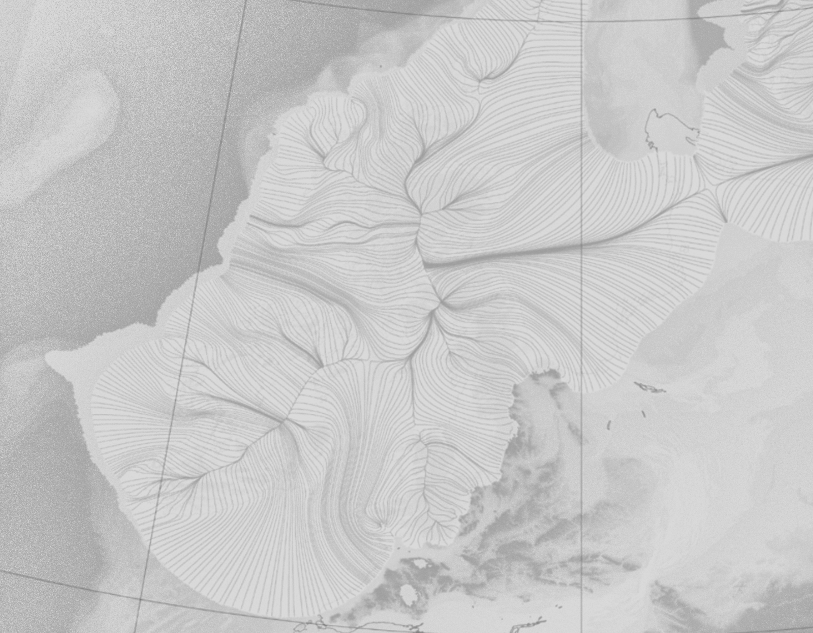
\includegraphics[width=\paperwidth]{images/gray-british-clark2022.png}}
  \begin{frame}
    \titlepage
  \end{frame}
}

\begin{frame}{Outline}
  \tableofcontents[hideallsubsections]
\end{frame}


\section{what is an ice sheet model?}

\begin{frame}{what is an ice sheet?}

\begin{itemize}
\item before numerical modeling \dots \emph{what} are we modeling?
\item \emph{def.} an \alert{ice sheet} is a large glacier with small thickness$/$width ratio
\end{itemize}

\bigskip
\begin{minipage}[t][60cm][t]{\textwidth}
\begin{center}
\includegraphics<1>[height=0.69\textheight]{images/ant-pittard2021.png}
\only<1>{\par {\scriptsize Antarctic ice sheet}} % (Pittard et al 2021)
\only<2>{\vspace{17mm}}
\includegraphics<2>[width=\textwidth]{images/ant-schoofhewitt2013.png}
\only<2>{\vspace{13mm}}
\only<2>{\par {\scriptsize note vertical exaggeration and rough bed (Schoof \& Hewitt 2013)}}
\includegraphics<3>[height=0.69\textheight]{images/alps-seguinot2018.png}
\only<3>{\par {\scriptsize modeled Alpine ice sheet near last glacial maximum (Seguinot et al 2018)}}
\includegraphics<4>[height=0.69\textheight]{images/british-clark2022.png}
\only<4>{\par {\scriptsize modeled British-Irish ice sheet near last glacial maximum (Clark et al 2022)}}
\includegraphics<5>[height=0.69\textheight]{images/not-sea-ice.png}
\only<5>{\par {\scriptsize but an ice sheet is \emph{not} sea ice!}}
\end{center}
\end{minipage}
\end{frame}


\begin{frame}{basic facts}

\begin{columns}
\begin{column}{0.6\textwidth}
\begin{itemize}
\item glacier ice is modeled as a \emph{slow, incompressible, viscous, non-Newtonian fluid}
    \begin{itemize}
    \item[$\circ$] more on that soon!
    \end{itemize}
\item ice sheet geometry and velocity evolve \emph{in contact with the climate}
    \begin{itemize}
    \item[$\circ$] snowfall
    \item[$\circ$] surface melt
    \item[$\circ$] subglacial melt
    \item[$\circ$] melt and calving when floating in the ocean (\emph{ice shelves})
    \end{itemize}
\end{itemize}
\end{column}
\begin{column}{0.42\textwidth}
\hfill 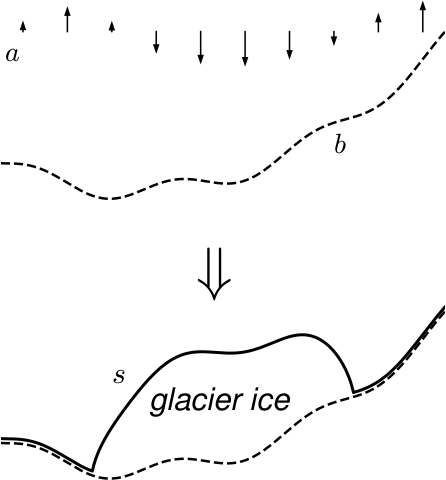
\includegraphics[width=0.9\textwidth]{images/map-glacier-ice.png}
\end{column}
\end{columns}
\end{frame}


\begin{frame}{what is an ice sheet model?}

\begin{columns}
\begin{column}{0.6\textwidth}
\begin{itemize}
\item for simplicity/clarity of the upcoming performance analysis, I will be ignoring quite a bit of physics!
\item \alert{ignoring}:
    \begin{itemize}
    \item[$\circ$] floating ice
    \item[$\circ$] subglacial hydrology
    \item[$\circ$] ice temperature
    \item[$\circ$] fracture processes (calving, crevasses)
    \item[$\circ$] solid earth deformation
    \end{itemize}
\item now, a simple definition of ``ice sheet model'' \dots
\end{itemize}
\end{column}
\begin{column}{0.42\textwidth}
\hfill 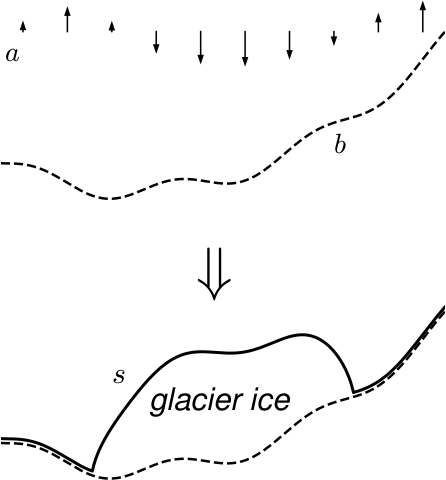
\includegraphics[width=0.9\textwidth]{images/map-glacier-ice.png}
\end{column}
\end{columns}
\end{frame}


\begin{frame}{what is an ice sheet model?}

\begin{columns}
\begin{column}{0.6\textwidth}
\begin{itemize}
\begin{definition}
an \alert{ice sheet model} is a \underline{map} which simulates an ice sheet in a climate
\end{definition} 
\item two inputs:
    \begin{itemize}
    \item[$\circ$] \emph{surface mass balance}
$$\hspace{-7mm} a(t,x,y) = \begin{pmatrix}
\text{balance of precipitation vs} \\
\text{melt \& runoff from surfaces}
\end{pmatrix}$$

\vspace{-3mm}
        \begin{itemize}
        \item[{\scriptsize $\bullet$}] units of mass flux:\, $\text{kg}\, \text{m}^{-2} \text{s}^{-1}$
        \end{itemize}

    \item[$\circ$] \emph{bed elevation} $b(x,y)$
    \end{itemize}
\item two outputs:
    \begin{itemize}
    \item[$\circ$] \emph{upper surface elevation} $s(t,x,y)$
    \item[$\circ$] \emph{ice velocity} $\bu(t,x,y,z)$
    \end{itemize}
\item {\small $\begin{pmatrix} \text{climate} \\ \text{topography} \end{pmatrix} \to \begin{pmatrix} \text{geometry} \\ \text{velocity} \end{pmatrix}$}
\end{itemize}
\end{column}
\begin{column}{0.42\textwidth}
\hfill 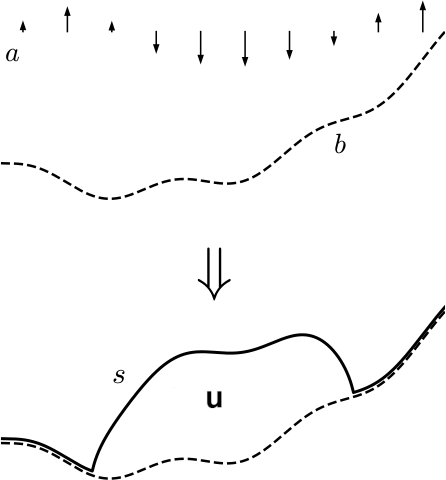
\includegraphics[width=0.9\textwidth]{images/map-velocity.png}

\vspace{2mm}
\end{column}
\end{columns}
\end{frame}


\begin{frame}{notation}

\begin{itemize}
%\item but this is a mathematics talk \dots notation! equations!
\item the data $a(t,x,y)$, $b(x,y)$ is defined on fixed time and space domains:
	$$t \in [0,T] \quad \text{and} \quad (x,y) \in \Omega \subset \RR^2$$

\begin{center}
\includegraphics<1>[width=0.55\textheight]{images/domain-data.png}
\includegraphics<2>[width=0.6\textheight]{images/domain-velocity.png}
\end{center}

\medskip
\item<2> the solution surface elevation $s(t,x,y)$ is defined on $[0,T]\times \Omega$
    \begin{itemize}
    \item[$\circ$] $s=b$ where there is no ice
    \end{itemize}

\item<2> one must \emph{solve} for the time-dependent \alert{icy domain} $\Lambda(t) \subset \Omega$ on which the velocity $\bu(t,x,y,z)$ is defined:
    $$\Lambda(t) = \left\{(x,y,z)\,:\,b(x,y) < z < s(t,x,y)\right\}$$

\vspace{-2mm}
    \begin{itemize}
    \item[$\circ$] $\Gamma_s(t),\Gamma_b(t) \subset \partial \Lambda(t)$ denote the surface and base of the ice
    \end{itemize}
\end{itemize}
\end{frame}


\begin{frame}{conservation}

\begin{itemize}
\item ice sheet evolution is a \alert{free-boundary conservation} problem
    \begin{itemize}
    \item[$\circ$] mass conservation
    \item[$\circ$] momentum conservation
    \item[$\circ$] energy conservation (\emph{ignored here})
    \end{itemize}
\item key idea: conservation of mass means both conserve mass in interior (incompressible) and at surface (SKE)
\end{itemize}
\end{frame}


\begin{frame}{strong form of ice sheet model}

\begin{itemize}
\item nonlinear complementarity problem coupled to Stokes:
\begin{align*}
s - b &\ge 0 && \text{on $\Omega \subset \RR^2$} \\
\frac{\partial s}{\partial t} - \bu|_s \cdot \bn_s - a &\ge 0 && \text{''} \\
(s - b) \left(\frac{\partial s}{\partial t} - \bu|_s \cdot \bn_s - a\right) &= 0 && \text{''} \\
- \nabla \cdot \left(2 \nu_\eps(D\bu)\, D\bu\right) + \nabla p - \rhoi \mathbf{g} &= \bzero && \text{on $\Lambda(t) \subset \RR^3$} \\
\nabla \cdot \bu &= 0 && \text{''} \\
\bu\cdot \bn = 0 \quad \& \quad \btau_b - \bbf(\bu) &= \bzero && \text{on $\Gamma_b(t) \subset \partial \Lambda(t)$} \\
\left(2 \nu_\eps(D\bu) D\bu - pI\right) \bn &= \bzero && \text{on $\Gamma_s(t) \subset \partial \Lambda(t)$}
\end{align*}

    \begin{itemize}
    \item viscosity by Glen law: \, $2\nu_\eps(D\bu) = \Gamma \left(|D\bu|^2 + \eps\, D_0^2\right)^{(\pp-2)/2}$
    \end{itemize}
\end{itemize}
\end{frame}


\section{time-stepping and stability}



\section{a simplified performance analysis}

\begin{frame}{complexity table}

%\setlength{\tabcolsep}{5pt}
%\renewcommand{\arraystretch}{1.5}

\begin{tabular}{llll}
\emph{time-stepping} & \emph{dynamics} & \emph{flops per model year} & \emph{[pessimistic stability]} \\ \hline
explicit & SIA    & $\oo{\frac{D\, L^2}{\Delta x^4}} = \oo{\frac{D\, m^2}{L^2}}$ \\
explicit & Stokes & $\oo{\frac{U L^{2+2\alpha}}{\Delta x^{3+2\alpha}}} = \oo{\frac{U m^{1.5+\alpha}}{L}}$ & $\oo{\frac{D\, L^{2+2\alpha}}{\Delta x^{4+2\alpha}}} = \oo{\frac{D\,m^{2+\alpha}}{L^2}}$ \\
implicit & SIA    & $\oo{\frac{q\, L^{2+2\beta}}{\Delta x^{2+2\beta}}} = \oo{q\, m^{1+\beta}}$ \\
implicit & Stokes & $\oo{\frac{q\, L^{2+2\gamma}}{\Delta x^{2+2\gamma}}} = \oo{q\, m^{1+\gamma}}$
\end{tabular}

\begin{itemize}
\item Asymptotic estimates of algorithmic scaling, measured by floating point operations per model year, for map-plane (2D) time-stepping numerical ice sheet simulations, in the high resolution limit where $\Delta x\to 0$ and $m\to\infty$
\end{itemize}
\end{frame}


\section{Stokes solver scaling}

\section{scalable implicit steps by multigrid?}

\begin{frame}{\alert{summary}}

\begin{itemize}
\item ice sheet models solve a multi-scale, irregular-data problem with hard-to-observe boundary conditions
   \begin{itemize}
   \item[$\circ$] there are \alert{no easy or magic techniques} for performance
   \end{itemize}
\item current-technology ice sheet models mostly use \alert{explicit time stepping}, \alert{non-optimal stress-balance solvers}, and shallow assumptions
\item \alert{coming soon} from current research:
   \begin{itemize}
   \item[$\circ$] scalable Stokes solvers (Isaac et al.~2015)
   \item[$\circ$] semi-implicit, semi-coupled time stepping (L{\"o}fgren et al.~2022)
   \item[$\circ$] ML emulators (Jouvet et al.~2021)
   \end{itemize}
\item scalable solvers for the implicit-step, coupled problem for ice sheet geometry requires advances in \alert{multilevel solutions of non-local variational inequalities}
\end{itemize}
\end{frame}


\begin{frame}{references}

\begin{itemize}
\footnotesize
\item E.~Bueler (2016). \emph{Stable finite volume element schemes for the shallow-ice approximation}, J.~Glaciol.~62 (232), 230--242, \href{https://doi.org/10.1017/jog.2015.3}{10.1017/jog.2015.3}
\item E.~Bueler (2021). \emph{Conservation laws for free-boundary fluid layers}, SIAM J.~Appl.~Math.~81 (5), 2007--2032, \href{https://doi.org/10.1137/20M135217X}{10.1137/20M135217X}
\item E.~Bueler (2022). \emph{Performance analysis of high-resolution ice-sheet simulations}, J.~Glaciol., \href{https://doi.org/10.1017/jog.2022.113}{10.1017/jog.2022.113}
\item T.~Isaac, G.~Stadler, \& O.~Ghattas (2015). \emph{Solution of nonlinear Stokes equations discretized by high-order finite elements on nonconforming and anisotropic meshes, with application to ice sheet dynamics}, SIAM J.~Sci.~Comput.~37 (6), B804--B833, \href{https://doi.org/10.1137/140974407}{10.1137/140974407}
\item G.~Jouvet, G.~Cordonnier, B.~Kim, M.~L\"uthi, A.~Vieli, A.~Aschwanden (2021). \emph{Deep learning speeds up ice flow modelling by several orders of magnitude}, J.~Glaciol.~\href{https://doi.org/10.1017/jog.2021.120}{10.1017/jog.2021.120}
\item A.~L{\"o}fgren, J. Ahlkrona, \& C. Helanow (2022). \emph{Increasing stable time-step sizes of the free-surface problem arising in ice-sheet simulations}, J.~Comput.~Phys.~X 16, \href{https://doi.org/10.1016/j.jcpx.2022.100114}{10.1016/j.jcpx.2022.100114}
\end{itemize}
\end{frame}




\end{document}
